\section{Modello XY}

%-----------------------------------------%
%				Prima slide				  %
%	   Caratterizzazione del modello   	  %
%-----------------------------------------%
\begin{frame}
    \frametitle{Caratterizzazione}
    \framesubtitle{}

    \begin{columns}
        \begin{column}{0.33\textwidth}
            \begin{block}{Termalizzazione}
            
            \end{block}
        \end{column}
    
        \begin{column}{0.33\textwidth}
            \begin{block}{Auto-correlazione}
            
            \end{block}
        \end{column}

        \begin{column}{0.33\textwidth}
            \begin{block}{Blocchi}

            \end{block}        
        \end{column}
    \end{columns}
\end{frame}



%-----------------------------------------%
%			  Seconda slide				  %
%	  Studio configurazioni low-highT  	  %
%-----------------------------------------%
\begin{frame}
    \frametitle{Configurazioni}
    \framesubtitle{}

    \begin{columns}
        \begin{column}{0.5\textwidth}
            \begin{block}{Bassa temperatura}

            \centering
            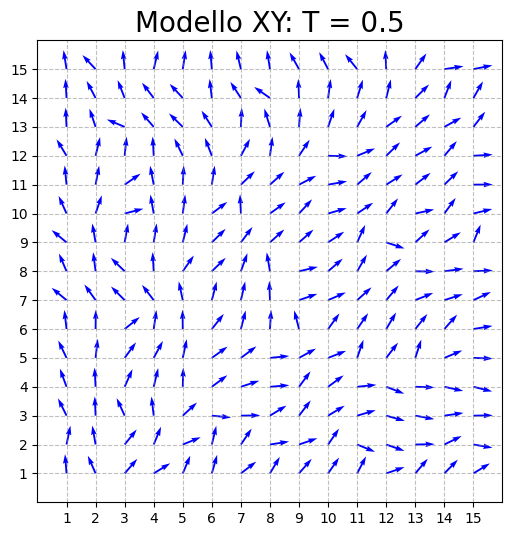
\includegraphics[width=0.8\textwidth]{Immagini/simXY/conf_T0.5.png}

            \end{block}
        \end{column}
    
        \begin{column}{0.5\textwidth}
            \begin{block}{Alta temperatura}

                \centering
                \includegraphics[width=0.8\textwidth]{Immagini/simXY/conf_T2.5.png}

            \end{block}
        \end{column}
    \end{columns}

\end{frame}



%-----------------------------------------%
%			   Terza slide				  %
%	       Esempio di vortice        	  %
%-----------------------------------------%
\begin{frame}
    \frametitle{Vortice}
    \framesubtitle{}

    \begin{columns}
        \begin{column}{0.5\textwidth}
            \centering
            %\includegraphics[width=0.8\textwidth]{Immagini/simXY/conf_vort.png}
        \end{column}
    
        \begin{column}{0.5\textwidth}
            \begin{itemize}[itemsep=0.5em, label=$\diamond$]
                \item Winding number $w\,=\,1$
                \item Transizione di Kosterlitz-Thouless
            \end{itemize}
        \end{column}
        \vspace{12pt}
        $T_c\,=\,\frac{\pi J}{2} $
    \end{columns}

\end{frame}



%-----------------------------------------%
%			   Quarta slide				  %
%	   Energia e Magnetizzazione XY  	  %
%-----------------------------------------%
\begin{frame}
    \frametitle{Osservabili}
    \framesubtitle{}

    \begin{columns}
        \begin{column}{0.5\textwidth}
            \begin{block}{Energia}

            \end{block}
        \end{column}
    
        \begin{column}{0.5\textwidth}
            \begin{block}{Magnetizzazione}

            \end{block}
        \end{column}
    \end{columns}

\end{frame}
